\documentclass[pdf,colorBG,slideColor]{prosper}
\hypersetup{pdfpagemode=FullScreen}

\usepackage{amsmath}
\usepackage{graphicx}

\newcommand{\itemt}[1]{\item {\bf #1} -}

\title{FASTlib}
\subtitle{A library of Fundamental Algorithmic and Statistical Tools}
\author{FASTlab}
\institution{College of Computing\\Georgia Institute of Technology}

\begin{document}

\maketitle

\begin{slide}{FASTlib}
 \vspace*{.6in}
 FASTlib is a new library for fast machine learning on large data sets.
\end{slide}

\begin{slide}{Mission}
 We aim to...
 \\
 \begin{itemize}
  \item Offer fast code for state-of-the-art algorithms in various machine learning fields.
  \item Make it easy for others to incorporate/understand/contribute to our work.
  \begin{itemize}
    \item Implies having a tolerable learning curve and encouraging distributed development.
  \end{itemize}
  \item Broaden our toolbox of methods for comparsion purposes.
  \item Experiment with new techniques.
 \end{itemize}
\end{slide}

\begin{slide}{Why not library X?}
 Some existing libraries:
 \begin{itemize}
  \itemt{Auton} Difficult to extend existing code without modifying it directly.
  Now a maintenance nightmare.
  \itemt{Frank Dellaert's OCaml library}
  Although alternative languages are faster than C++ some of the time,
  sometimes they are unacceptably slow for a performance-oriented group.
  \itemt{Weka} Large class hierarchies are bad for old-school developers.
  We can discuss Java's performance limitations.
 \end{itemize}
\end{slide}

\begin{slide}{How Can FASTlib Be Better?}
 \begin{itemize}
  \itemt{Design} Use well-thought-out, flexible designs with an eye for future extension.
  Avoid over-complicated designs that serve no purpose, even if they ``sound neat on paper''.
  (The ``KISS'' principle.)
  \itemt{Documentation} Document as much as reasonable.
  Avoid ``I have no idea why that code works -- don't touch it''.
  Includes in-code and wiki-based documentation.
  \itemt{Debugging} Machine learning algorithms can produce results from garbage -- to compensate, we have strong debugging support.
  \itemt{Speed} Be fast, but avoid pitfalls of low-level development.
  \itemt{Testing} Significant components should provide tests.
 \end{itemize}
\end{slide}

\begin{slide}{Why Can FASTlib Be Better?}
 \begin{itemize}
  \itemt{Knowledge} Lots of experiences with Auton's weaknesses.
  \itemt{Diversity and Integration}
  Centralized respository but decentralized development allows one cohesive unit with many diverse components.
  \itemt{Language Features}
  We choose a powerful language but use it wisely.
  \itemt{Specialized} It's our library, for statistical machine-learning purposes, and we control it.
 \end{itemize}
\end{slide}

\begin{slide}{Separation}
 FASTlib is divided into two main parts:
 \begin{itemize}
 \itemt{Core} What this presentation describes.  This part can be built by
 the community but will have much stricter standards.
 \itemt{Arsenal} Collaborateively-built standalone algorithms.
 This is what you will probably work on!
 \end{itemize}
 Everyone will have read/write access to a Subversion repository with both.
\end{slide}

\begin{slide}{Language}
 C++ is our language of choice:
 \begin{itemize}
 \itemt{Popular} Well-known even among non-CS, and reasonably portable.
 \itemt{Fast} Low-level, low-overhead with direct machine control.
 \itemt{High-Level} Enough to allow widespread code reuse.
 \end{itemize}
 Python is our scripting language of choice.
 (You won't have to worry about Makefiles.)
\end{slide}

\begin{slide}{Design Decisions}
 After a month of debate, we decided:
 \begin{itemize}
  \itemt{Shallow Class Hierarchies}
  Avoid unnecessary object-oriented abstraction.
  \itemt{Ease/Power Duality}
  Simple solutions for simple scenarios, but have separate ``power user'' features available.
  \itemt{Default Constructors with Explicit Initializers}
  Allows for greater control over object lifecycle.
  We compensate with good debugging checks.
  \itemt{C-like Feel}
  Many OO principles hinder rapid development algorithmic code.
  OO is only used on components that need it\footnote{A {\tt class} does not OO make -- think virtual methods and design patterns.}.
 \end{itemize}
\end{slide}

\begin{slide}{Main Packages}
 \begin{tabular}{rl}
   {\bf Debug/Base}    & Bare necessities. \\
   {\bf FASTexec}      & Parameters, timers, results, and automation. \\
   {\bf Datasets}      & Reading/writing/accessing mixed data. \\
   {\bf Collections}   & Dynamic arrays and other storage classes. \\
   {\bf Math}          & Kernels, metrics, etc.; eventually more. \\
   {\bf Linear Alg}    & An interface for LAPACK. \\
   {\bf Spatial Trees} & Formation and utilities. \\
   {\bf THOR}          & Parallel dual-tree algorithms.
 \end{tabular}
\end{slide}

\begin{slide}{Features - Base}
 Debug/Base ({\tt base}):
 \begin{itemize}
 \itemt{Runtime Checks} Low-overhead bounds checks and assertions.
 \itemt{Debug Mode} Checks can be disabled with a simple switch.
 \itemt{Performance Directives} Compiler directives to assist the compiler.
 \itemt{Object Traversal (OT)} Abstract serialization, deserialization, and debug printing.
 \end{itemize}
\end{slide}

\begin{slide}{Features - FASTexec}
 FASTexec ({\tt fx}):
 \begin{itemize}
 \itemt{Modular Storage} Hierarchical storage of parameters, results, and timers.
 \itemt{Parameters} Modular command-line parameters.
 \itemt{Experimental Conditions}
   Automatically records system information and usage info.
 \itemt{Data Extraction} Python scripts scan the output, making tables and charts.
 \end{itemize}
 \vspace{-.2in}
  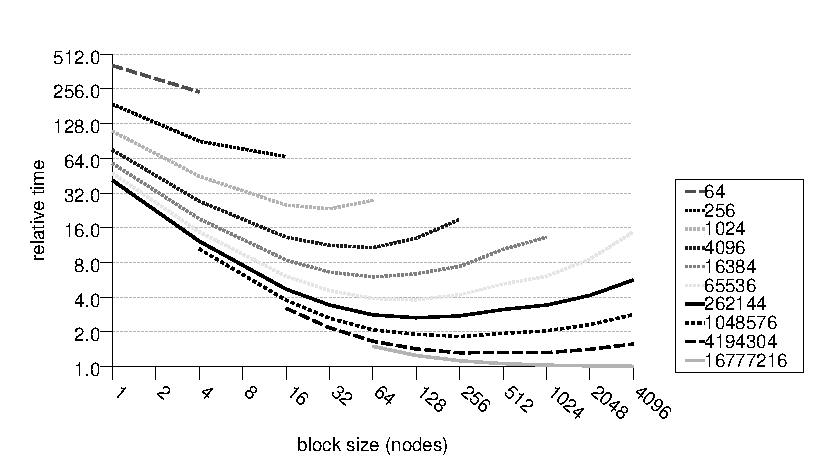
\includegraphics[width=2.2in]{g_blocksizes_t.ps}
  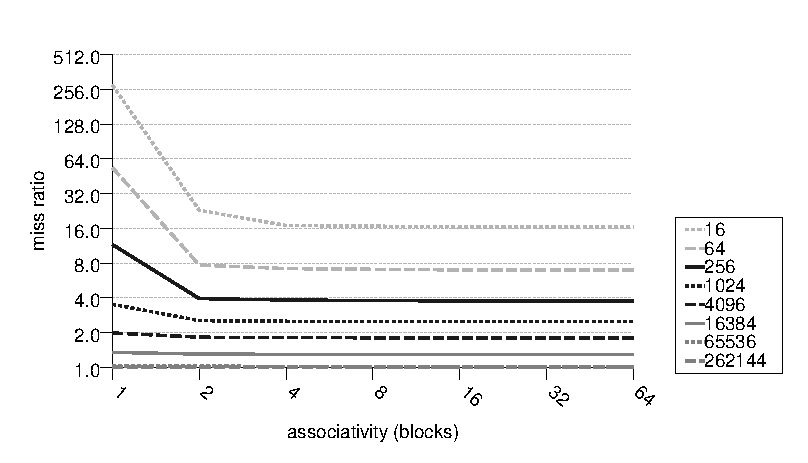
\includegraphics[width=2.2in]{g_assoc.ps}
\end{slide}

\begin{slide}{Features - Datasets}
 Datasets ({\tt data}):
 \begin{itemize}
 \itemt{Double-Precision Storage} Data stored as a matrix of doubles.
 \itemt{Multiple Representations} Features may be continuous, integral, or nominal.
 \itemt{Column-Major} A datum is a column, for FORTRAN/LAPACK support.
 \itemt{Text Formats} Reads/writes {\tt arff} and {\tt csv}
 \itemt{Aliasing} Non-copying access to column vectors and submatrices.
 \itemt{Cross-Validation} Randomized or strided cross validation.
 \end{itemize}
\end{slide}

\begin{slide}{Features - Collections}
 Collections ({\tt col}):
 \begin{itemize}
 \itemt{ArrayList} Templated dynamic array, works with library standards.
 \itemt{Queues} Priority and FIFO queues.
 \itemt{Miscellanous} Range sets, and dense integer map.
 \item More to come later, but C++ also has a wide variety of STL classes.
 \end{itemize}
\end{slide}

\begin{slide}{Features - Linear Algebra}
 Linear Algebra ({\tt la}):
 \begin{itemize}
 \itemt{Matrices, Vectors} Compatible with dataset classes.
 \itemt{LAPACK Wrappers} Easy-to-use LAPACK wrappers.
 \itemt{LAPACK Support}
 Supports custom built ATLAS, or builds reference implementation automatically.
 \end{itemize}
 \vspace*{.2in}
 Spatial Trees ({\tt tree}):
 \begin{itemize}
 \itemt{Abstract} Trees have abstract bounding types.
 \itemt{Building} Currently, builds KD-trees.
 \itemt{Statistics} Tempated statistics computed for nodes
 \end{itemize}
\end{slide}

\begin{slide}{Features - Math}
 Other Math ({\tt math}): \\
 \begin{itemize}
 \item Various tools for discrete math, geometry, etc.
 \item Gaussian and Epanechnikov kernels.
 \item Great opportunity for extension, hint hint
 \end{itemize}
\end{slide}

\begin{slide}{Code Example - Main}
 \vspace*{.3in}
 We will write a {\tt main()} that: \\
 \begin{itemize}
 \item Does cross-validation on a KNN classifier.
 \item Accepts parameters for number of cross validation folds and number
 of nearest neighbors: \verb|./main --kfold/k=10 --knn/k=5 --fname=q.arff|
 \item Builds by: \verb|fl-build main|
 \item Yields results and timers for everything, for example:
\begin{verbatim}
/kfold/results/p_correct 0.805
/kfold/timers/total/wall/sec 0.025244
\end{verbatim}
 \end{itemize}
\end{slide}

\begin{slide}{Code Example - Main}
 {\tt main()} for K Nearest Neighbors classifier:
 \vspace*{.1in}
\begin{verbatim}
#include "knn.h"
#include "fastlib/fastlib.h"
int main(int argc, char *argv[]) {
 fx_init(argc, argv);
 const char *fname =
     fx_param_str(fx_root, "fname", NULL);
 Dataset dataset;
 dataset.InitFromFile(data);
 SimpleCrossValidator<KnnClassifier> xvd;
 xvd.Init(&dataset, 0, 10, fx_root, "knn");
 xvd.Run();
 fx_done();
}
\end{verbatim}
\end{slide}

\begin{slide}{Code Example - Building}
 Build file ({\tt build.py}) for previous example, located in
 the same directory as source code {\tt main.cc}:
 \vspace{0.05in}
\begin{verbatim}
  binrule(
      name = "main",
      sources = ["main.cc"],
      deplibs = ["fastlib:fastlib"])

  $$ fl-build main
\end{verbatim}
 \vspace{0.05in}
 If all you need is core FASTlib, you can skip the build file:
 \vspace{0.05in}
\begin{verbatim}
  $$ fl-build main.cc
\end{verbatim}
 \vspace{0.05in}
 Other options:
\begin{verbatim}
  $$ fl-build main --mode=fast --cflags="-DXYZ"
  $$ make clean
\end{verbatim}
 
\end{slide}

\begin{slide}{Code Example - 1 Nearest Neighbor}
 \vspace{-.17in}
\begin{verbatim}
int OneNNClassifier::Classify(
   const Vector& test) {
 double closest = DBL_MAX; double label = -1;
 index_t d = matrix_.n_cols()-1; // dimension
 for (index_t i = 0; i<matrix_.n_cols(); i++){
  Vector train;
  matrix_.MakeColumnSubvector(i,0,d,&train);
  double dist_squared =
      la::DistanceSqEuclidean(test, train);
  if (unlikely(dist_squared < closest)) {
    closest = dist_squared;
    label = matrix_.get(i, d);
  }
 }
 return int(label);
}
\end{verbatim}
\end{slide}

\begin{slide}{Code Example - SVD}
\vspace{-.17in}
\begin{verbatim}
 Matrix A, U, VT, S, tmp, new_A;
 Vector s;

 data::Read("foo.csv", &A);
 la::SVDInit(A, &s, &U, &VT);
 S.InitDiagonal(s);
 la::MulInit(U, S, &tmp);
 la::MulInit(tmp, VT, &new_A);
 //.. new_A should equal A
\end{verbatim}
\end{slide}

\begin{slide}{Code Example - Modules}
\vspace{-.17in}
\begin{verbatim}
void DoCache(datanode *module,
             ArrayList<int> *perm) {
  int n = fx_param_int_req(module, "n");
  fx_timer_start(module, "permute");
  if (fx_param_bool(module, "random", 0)) {
    math::MakeRandomPermutation(n, perm);
  } else {
    math::MakeIdentityPermutation(n, perm);
  }
  fx_timer_stop(module, "permute");
}
void DoBoth(datanode *module) {
  ArrayList<int> a, b;
  DoCache(fx_submodule(module, "a", "a"), &a);
  DoCache(fx_submodule(module, "b", "b"), &b);
}
\end{verbatim}
\end{slide}

\begin{slide}{Code Example - Modules (cont.)}
\vspace{-.17in}
\begin{verbatim}
int main(int argc, char *argv[]) {
  fx_init(argc, argv);
  DoBoth(fx_root);
  fx_done();
}

$$ ./main --a/random=false --a/n=10000000
          --b/random=true --b/n=10000000

/a/params/n 10000000
/a/params/random false
/a/timers/permute/wall/cycles 177184032
/a/timers/permute/wall/sec 0.111000
/b/params/n 10000000
/b/params/random true
/b/timers/permute/wall/sec 1.953043
\end{verbatim}
\end{slide}

%\begin{slide}{Code Example}
%  \vspace*{.3in}
%  The last example: \\
%  \begin{itemize}
%  \item Accepts parameters for number of cross validation folds and number
%  of nearest neighbors: \verb|./main --kfold/k=10 --knn/k=5 --data=q.arff|
%  \item Builds: \verb|fl-build main --mode=fast|
%  \item Yields results (and timers for everything):
%\begin{verbatim}
%/kfold/results/p_correct 0.805
%/kfold/timers/total/wall/sec 0.025244
%\end{verbatim}
%  \end{itemize}
%\end{slide}
%
%\begin{slide}{Code Example - 1 Nearest Neighbor}
%\begin{verbatim}
%  for (index_t i = 0; i < matrix_.n_cols(); i++) {
%    Vector train_wlabel;
%    Vector train;
%    double dist_squared;
%    matrix_.MakeColumnVector(i, &train_wlabel);
%    train_wlabel.MakeSubvector(0,
%        matrix_.n_rows() - 1, &train);
%    dist_squared = la::DistanceSqEuclidean(
%        test, train);
%    if (unlikely(dist_squared < closest)) {
%      closest = dist_squared;
%      label = int(train_wlabel[
%          train_wlabel.length()-1]);
%    }
%  }
%\end{verbatim}
%\end{slide}

\begin{slide}{How do I start coding?}
 \vspace*{.3in}
 Ample resources should be available: \\
 \begin{itemize}
 \itemt{Tutorial} FASTlib's Tutorial on the wiki is the all-in-one guide to starting out.
 \itemt{Cookbook}
 For common tasks, we'll collaboratively contribute to a "cookbook" on the wiki.
 \itemt{Doxygen}
 Inline source documentation with Doxygen, a Javadoc-like tool.
 http://www-static.cc.gatech.edu/\~~garryb/fastlib/html
 \itemt{Email}
 The FASTlib developers are just an email away.
 \end{itemize}
\end{slide}

\end{document}
